\documentclass{automatextcc}
\usepackage{graphicx} % Para importar figuras
\usepackage{float} % Para posicionar as figuras de forma mais conveniente
\graphicspath{{figuras/}}

\begin{document}
%título do trabalho
\title{DESENVOLVIMENTO DE UM SISTEMA WEB PARA Agendamento em Barbearias e Salões de Beleza}
%autor do trabalho
\author{xxxa}
%orientador(a) do trabalho {nome}{Orientador(a)}
\advisor{Profa. Dr. xxx}{Orientador(a)}
%universidade onde obteve o título e atual
\advisorinfo{Doutor(a) pela xxx, PR}{XXX}
%outro exemplo
%\advisor{Prof. Dr. Heraldo José de Amorim}{Orientador}
%\advisorinfo{Doutor pela \ufrgs~--~Porto Alegre, RS}{UFRGS}
%banca examinadora:

%banca examinadora:
\examinera{Prof. Dr. xxx}
\examinerainfo{Doutor pela Universidade Federal de XX XXX, PR}{XXXX}
\examinerb{Prof. Dr. xxx}
\examinerbinfo{Doutor pela Universidade Federal de XX XXX, PR}{XXXX}
\examinerc{Prof. Dr. xxx}
\examinercinfo{Doutor pela Universidade Federal de XX XXX, PR}{XXXX}

%departamento:
\dept{\DELAE}
%\dept{\DEMEC}
%\dept{|DELET}
%data de entrega
\date{Novembro de 2015}
%cria a capa

%banca examinadora:
\examinera{Prof. Dr. xxx}
\examinerainfo{Doutor pela Universidade Federal de XX XXX, PR}{XXXX}
\examinerb{Prof. Dr. xxx}
\examinerbinfo{Doutor pela Universidade Federal de XX XXX, PR}{XXXX}
\examinerc{Prof. Dr. xxx}
\examinercinfo{Doutor pela Universidade Federal de XX XXX, PR}{XXXX}
\maketitle
%agradecimentos
\chapter*{Agradecimentos}
Agradeço a todos que participaram xxx.

%palavras chave - português
\keyword{Salão de beleza}
\keyword{Software Web}
\keyword{NodeJS}
\keyword{metodologia XP}
%palavras chave- inglês
\keyworde{Beauty salon}
\keyworde{Web Software}
\keyworde{NodeJS}
\keyworde{XP methodology}

%resumo
\begin{abstract}
HENRIQUE ZAMBELI, Erik. Desenvolvimento de um sistema para agendamento em barbearias e salões de beleza. Proposta de Trabalho de Conclusão de Curso – Engenharia de Software, Universidade Tecnológica Federal do Paraná. Cornélio Procópio, 2018.

Com o enorme crescimento de barbearias e salões de beleza no Brasil se manter atualizado e gerenciar com cada vez mais eficiência o seu negócio se tornou essencial para se manter no mercado de trabalho. Como cada vez mais as pessoas estão tendo acesso a rede de computadores manter o seu estabelecimento gerenciável e online é essencial, disponibilizando assim transparência e agilidade ao consumidor final. Além de poder explorar novas possibilidades como os “barbershop” que necessitam de uma estrutura maior e mais gerenciável para manter o lucro. Diante disso este trabalho resultou no desenvolvimento de uma ferramenta web para gerenciamento de recursos, base de dados histórica de clientes e agendas de serviço online, e possibilitou dessa forma aplicar as técnicas, linguagens de programação e algumas ferramentas para melhorar a escalabilidade em servidores, como o caso da utilização do NodeJs, que além de fornecer componentes ricos, também disponibiliza recursos que torna o “backand” de uma aplicação mais eficiente.

\end{abstract}

%abstract


\begin{englishabstract}

HENRIQUE ZAMBELI, Erik. Development of a system for scheduling in barbershops and salons. Proposed Course Completion Work - Software Engineering, Federal Technological University of Paraná. Cornélio Procópio, 2018.

With the tremendous growth of barbershops and beauty salons in Brazil staying up to date and managing with ever more efficiency your business has become essential to staying in the job market. As more and more people are having access to computer network keeping their establishment manageable and online is essential, thus providing transparency and agility to the end consumer. In addition to being able to explore new possibilities such as "barbershop" that need a larger and more manageable structure to maintain profit. This work resulted in the development of a web tool for resource management, historical customer database and online service agendas, and made it possible to apply techniques, programming languages and some tools to improve server scalability, such as the case of the use of NodeJs, which in addition to providing rich components, also provides resources that makes the backand of an application more efficient.

\end{englishabstract}


%sumário
\tableofcontents
% lista de ilustrações
\listoffigures
% lista de tabelas
\listoftables
% lista de abreviaturas e siglas em ordem alfabética
% o parametro deve ser a abreviatura mais longa
\begin{listofabbrv}{ANABEL}
        \item[CSS] Cascading Style Sheets
        \item[HTML] Hypertext Markup Language
        \item[JS] JavaScript
        \item[MVC] Model View Controller
        \item[XP] Extreme Programming
        \item[TDD] Test-driven development
        \item[CRC] Use Class, Responsibilities, and Collaboration
        \item[DOM] Document Object Model
        \item[SGBD] Sistema de Gerenciamento de Banco de Dados
        \item[GNU] Gnu's Not Unix
        \item[JSON] JavaScript Object Notation
        \item[W3C] World Wide Web Consortium
        \item[SMS] short message service
         \item[SEBRAE] Serviço Brasileiro de Apoio às Micro e Pequenas Empresas
          \item[ANABEL] Associacao Nacional Do Comercio De Artigos De Higiene Pessoal E Beleza
\end{listofabbrv}
% lista de símbolos em ordem alfabética (opcional)
%\begin{listofsymbols}{}

%\end{listofsymbols}
%%%%%%%%%%%%%%%%%%%%%%%%%%%%%%%%%%%%%%%%%%%%%%%%%%%%%%%%%%%%%%%%%%%%%%%%%%%%%%%%
%COMEÇA O TEXTO DO TRABALHO DE CONCLUSÃO
%%%%%%%%%%%%%%%%%%%%%%%%%%%%%%%%%%%%%%%%%%%%%%%%%%%%%%%%%%%%%%%%%%%%%%%%%%%%%%%%
\chapter{Introdução}


\section{Motivação}
Beleza significa qualidade, virtude do que é belo, pode ser descrito como coisa que desperta o êxtase. O que torna a busca pela beleza um amplo e vasto mercado, com leque imenso de segmentos a ser explorado comercialmente, e um desses mercados é o ramo de salão de beleza e barbearias.

  	Segundo os dados da Juntas Comerciais do Brasil, existem em atividade no Brasil cerca de 600 mil estabelecimentos ligado ao ramo de beleza. No país o número de salões cresceu 78\% em cinco anos, segundo levantamento da Associação Nacional do Comércio de Artigos de Higiene Pessoal e Beleza (Anabel). Os salões de beleza se multiplicaram na época em que nossa economia crescia sem parar, e mesmo agora continuam surgindo novos salões.
  	Segundo o Sebrae [SEBRAE, 2016], muitas pessoas são frequentadores assíduos de salão de beleza e tem seus profissionais e estabelecimentos prediletos. Sejam negócios informais ou não, pequenos ou grandes centros estéticos, esse ramo possui bastante espaço para empresas e empreendedores que trabalham com qualidade e investem em diferenciais competitivos.
  	
 	Cerca de 7 mil salões são abertos por mês em todo território nacional, a maioria como microempreendedores individuais. Considerando-se o alto nível de informalidade destas atividades, estima-se que esses números trazidos a realidade, ultrapassaria a casa de um milhão de estabelecimentos em todo o país.
 	
 	Com o elevado crescimento desse ramo, há aspectos que impulsionaram o crescimento desse setor, como o acesso das classes ‘C’, ‘D’ e ‘E’, a participação cada vez maior da mulher no mercado de trabalho, lançamentos constantes de novos produtos visando um melhor atendimento das necessidade de mercado, o aumento da expectativa de vida, dentre outros, só fizeram elevar de patamar os salões de beleza e a necessidade de novas técnicas que auxiliem no bom funcionamento desses estabelecimentos, para que o elevado grau de informalidade, precariedade de funcionamento, não elevem as taxas de mortalidade dos negócios.


\section{Objetivos}

O projeto tem como objetivo geral realizar a otimização do processo de agendamento para um Salão de Beleza. O software irá realizar o agendamento de uma forma que otimiza o tempo médio gasto e preservar a integridade dos dados dos clientes e atendentes cadastrados, sendo um produto fácil e intuitivo de se usar. O software permitirá o cadastramento dos dados dos atendentes e clientes, cadastrar um cliente em determinado horário e relatar observações sobre o mesmo cliente. Ainda deve prover uma visualização de gargalos de serviços apresentados pelos relatório de apontamentos realizados pelos atendentes.

\subsection{Objetivos Gerais}

\begin{itemize}
\item Promover a otimização da agenda do negócio.

\item Organizar a base histórica dos clientes. 

\end{itemize}

\subsection{Objetivos Específicos}

\begin{itemize}
\item Monitorar em tempo real os recursos do negócio.

\item Acompanhar o andamento dos processos e avaliar os recursos mais sobrecarregados e ociosos do negócio.

\item Analisar o rendimento de cada funcionário.

\item Armazenar o histórico de relacionamento de cada cliente.

\item Apontamento de serviço:  início, fim, paradas e esperas.

\end{itemize}

\section{Organização do documento}

O capitulo 1 aborda de maneira superficial o problema que a ferramenta se propõe a solucionar, traz as motivações e os principais objetivos a se alcançar durante o desenvolvimento.

O capitulo 2 aborda a base teórica por traz do software, além de expor trabalhos parecido e conceitos que serão utilizados no desenvolvimento.

O 3 capitulo trata das ferramentas que serão utilizadas no desenvolvimento além de aborda a metodologia que será utilizada no desenvolvimento do trabalho.

No ultimo capitulo, e apresentado uma pequena tabela do cronograma de desenvolvimento do trabalho.


\chapter{Fundamentação Teórica}

Este capítulo explica os conceitos que dão base ao projeto e todas as tecnologias que serão utilizadas no desenvolvimento. Ainda neste capítulo serão apresentados os trabalhos correlatos.


\section{Referencial Teórico}


\section{Trabalhos Correlatos}

Nesta seção, é apresentada uma visão geral sobre trabalhos relacionados ao escopo proposto por este projeto.

Hoje no Brasil existem inúmeros softwares neste segmento, afinal ter um sistema informatizado pode auxiliar e muito no dia a dia. Várias opções são oferecidas como a que permite todo o controle de clientes, fluxo de caixa e outros procedimentos que são executados sempre na rotina de salão de beleza.

São eles:

\subsection{Software Beleza Soft}

O “Beleza Soft”, que é um dos mais famosos softwares para salão de beleza, essa opção é ideal para quem quer ter um programa fácil de gerenciar e alimentar, não é necessário nenhum conhecimento específico anteriormente.

   Comanda sistema Beleza Soft imagem \ref{img4}: 
 \begin{figure}[h!]
    \centering
	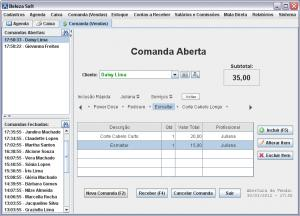
\includegraphics[scale=1]{comanda}
	\caption{Comanda sistema Beleza Soft}
	\label{img4}
\end{figure}

Se trata de uma ferramenta desktop é sua principal funcionalidade e abrir uma comanda para cada cliente cadastrado, nesta comanda e possível marcar quais serviços serão prestados ao cliente e o valor de cada serviço assim como o funcionário que irá prestar o serviço. Ao final do atendimento a comanda e fechada e o valor a pagar e informado ao usuário. O sistema ainda possui um controle de caixa que permite gerar um relatório de serviços prestados de fluxo de caixa e gasto com profissionais. 


\subsection{Software CPT Salão de Beleza}

O “CPT Salão de Beleza” se trata de uma ferramenta desktop, esse software não é exclusivo para salões de beleza, pode ser usado no ramo da estética, como clínicas de massagens, e estética corporal, entre as suas funcionalidades estão: além de itens básicos como cadastro, esse software exibe avisos automáticos de estoque mínimo de produtos cadastrados, boletos a vencer, além de apontar o aniversariante do dia.

  Agenda CPT Salão de Beleza imagem \ref{img6}: 
 \begin{figure}[h!]
    \centering
	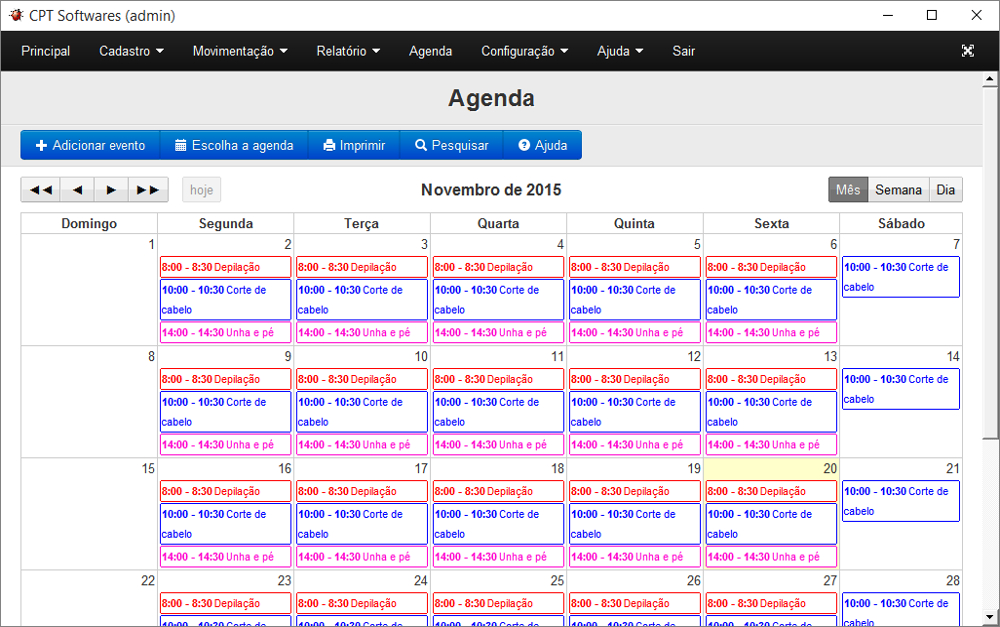
\includegraphics[scale=0.3]{agenda-salao}
	\caption{Agenda CPT Salão de Beleza }
	\label{img6}
\end{figure}

\subsection{Software Salão Vip}

O “Salão Vip”  e uma ferramenta paga que tem como uma de suas vantagens não precisa ser instalado no computador para ser executado, ele usa computação em nuvem, uma tendência que já vem sendo dominante no mercado de serviços de softwares, entre suas funcionalidades estão: controle dos itens que são consumidos pelo salão, esse software possui também uma ferramenta de relacionamento entre cliente e funcionário, comunicando através de mensagens SMS, e-mail marketing.

   Comanda Salão Vip imagem \ref{img7}: 
 \begin{figure}[h!]
    \centering
	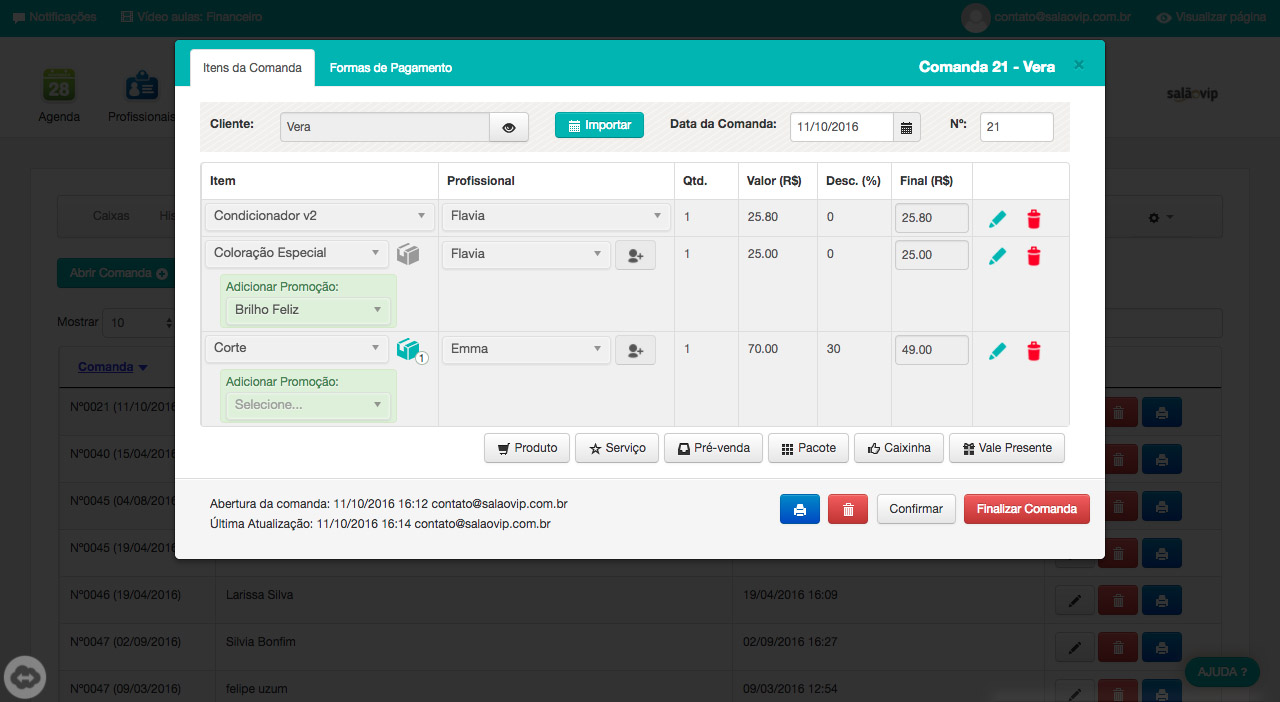
\includegraphics[scale=0.24]{comandaVip}
	\caption{Comanda Salão Vip}
	\label{img7}
\end{figure}

\chapter{Materiais e Métodos}

Este capitulo apresenta os materiais e as metodologias que serão utilizadas durante o desenvolvimento do projeto.

\section{Materiais}
    
Os materiais utilizados no desenvolvimento do sistema proposto foram:

\subsection{HTML 5}

Apresentado pela W3C (2017c) HyperText Markup Language (HTML), cuja versão atual é 5, é uma linguagem de marcação simples, baseada em texto e de fácil aprendizagem que pode ser interpretada por qualquer navegador Web básico. Qualquer página da Web requer um mínimo de Html, caso contrário não seria uma página Web. 

O Html surgiu em meados de 1990 como um documento curto que detalhava uma gama de elementos utilizados para construção de páginas Web. Muitos desses elementos eram para descrever o conteúdo da página, tal como cabeçalhos, parágrafos e listas. Os números das versões do Html aumentaram de acordo com a evolução da linguagem e com a introdução de outros elementos e ajustes nas regras da linguagem. 

Html 5 é a evolução natural de suas versões anteriores e que se esforça para atender as necessidades atuais e futuras dos Websites. A versão 5 herda uma grande maioria das características de seus predecessores, o que significa que a linguagem é compatível tanto com navegadores antigos quanto navegadores novos. Ser compatível com versões anteriores é um princípio-chave do Html 5. 



\subsection{CSS 3}

De acordo com W3C (2017b), Cascading Style Sheets (CSS), atualmente na versão 3, é uma linguagem de folhas de estilo utilizada para definir a apresentação de documentos escritos em uma linguagem de marcação (HTML por exemplo). O CSS surgiu após o Html estar no mercado após alguns anos, se tornando oficial em 1996. O CSS 3, assim como Html 5, é uma evolução natural dos seu antecedores. CSS 3 é muito mais poderoso do que suas versões anteriores, e introduz uma grande variedade de efeitos visuais, tais como sombras, cantos arredondados e gradientes. De maneira geral, CSS é utilizado para dar cores e outros tipos de edições visuais na página Web.


\subsection{JavaScript}

JavaScript é uma linguagem de script de objetos inventada por Brendan Eich em 1995 e utilizada em milhões de páginas Web e aplicações de servidores mundialmente. MDN (2017) define ECMA-262 é o nome oficial do Javascript e a versão mais atual é o ECMAScript 6, lançado em junho de 2015. Ao contrário da crença popular que JavaScript é “Java interpretado”, JavaScript, de maneira geral, é uma linguagem de script dinâmica que oferece suporte à construção de objetos baseados em protótipos. 

\subsection{Node.js}

Node.js é um interpretador de código JavaScript com o código aberto, focado em migrar o Javascript do lado do cliente para servidores. Seu objetivo é ajudar programadores na criação de aplicações de alta escalabilidade, com códigos capazes de manipular dezenas de milhares de conexões simultâneas, numa única máquina física.

O Node.js roda uma programação assíncrona, sem bloqueio, de encadeamento único, que é muito eficiente em termos de memória.


\subsection{MongoDB}

O desenvolvimento de MongoDB começou em outubro de 2007 pela 10gen, atual MongoDB Inc., e sua primeira versão pública foi lançada em fevereiro de 2009.  É um software de banco de dados orientado a documentos livre, de código aberto e multiplataforma, escrito na linguagemC++. Classificado como um programa de banco de dados NoSQL, o MongoDB usa documentos semelhantes a JSON com esquemas. É desenvolvido pela MongoDB Inc. e publicado sob uma combinação da GNU Affero General Public License e Licença Apache.

Suas características permitem com que as aplicações modelem informações de modo muito mais natural, pois os dados podem ser aninhados em hierarquias complexas e continuar a ser indexáveis e fáceis de buscar.


\subsection{ReactJS}

React é uma ferramenta somente para criar componentes. Criada pela equipe do Instagram entrou para o lista de projetos open-source do Facebook, que  impulsionando mais ainda sua adoção. O grande sucesso do React se deve ao Virtual-DOM.

Virtual-DOM é uma técnica de representação em JavaScript puro do DOM “real” em memoria. A manipulação do DOM e algo extremamente dificil e causa vários problemas na sua aplicação. Com v-dom passa-se a manipular esse objeto e não o DOM real. Quando o objeto v-dom é atualizado um algoritmo calcula a diferença entre o v-dom e o DOM real, alterando então pedaços de DOM real.

\subsection{ Bootstrap 3.0}

Bootstrap, de acordo com W3C (2017a), é uma framework front-end elegante, intuitivo e poderoso para desenvolvimento Web mais rápido e prático, criado por Mark Otto e Jacob Thornton, e mantido por uma equipe principal com apoio e envolvimento maciço da comunidade de desenvolvedores Web. A versão utilizada neste trabalho foi a versão 3.0.

\subsection{jQuery}

jQuery é uma biblioteca JavaScript pequena, rápida e cheia de funcionalidades. A utilização do jQuery faz com que atividades de travessia e manipulação de documentos Html, manipulação de eventos, animações e AJAX sejam executadas de maneira muito mais simples com uma Interface de Aplicação de Programação (API) fácil de usar e que funciona na grande maioria dos navegadores Web. 

\subsection{Google Chrome}

Google Chrome é um navegador para internet, criado pela Google, combina tecnologias sofisticadas com um design simples para tornar a Web mais rápida, mais segura e mais prática. (GOOGLE, 2014) Um dos recursos que essa ferramenta possui e foi utilizado no decorrer do desenvolvimento do sistema proposto, é o recurso de inspeção de código. Com ele foi possível escolher características visuais para o sistema, depurar códigos e acompanhar algumas funcionalidades.

\subsection{Model Viewer Controller(MVC)}

Model Viewer Controller (MVC), de acordo com SILVA (2012), é um padrão que sugere uma arquitetura de software dividi da em componentes, de forma a viabilizar com clareza o desenvolvimento de um código enxuto e mais organizado, que por sua vez facilita a reciclagem e manutenção do sistema de maneira fácil e segura. Entretanto, para que a independência dos componentes seja atingida deve haver uma organização do sistema em  camadas, garantindo a escalabilidade, re-usabilidade e eficiência dos componentes. SILVA (2012) ainda define que a separação de componentes visa primariamente separar  a lógica do sistema da interface do usuário. 

As camadas Model(Modelo), Viewer (Visão) e Controller(Controle) exercem esta divisão de funcionalidades sendo que, no padrão MVC, o Model trabalha na manipulação dos dados internos da aplicação e se comunica especialmente como armazenamento dos dados. Já a camada de Viewer trabalha  diretamente a interface do usuário, controlando suas ações e enviando mensagens aos  Controllers, que, por meio dos modelos, acessamos dados e aplica a apresentação desses  dados conforme o evento. A camada de Controllers por sua vez exerce funcionalidades que definem o comportamento da aplicação, sendo responsáveis pelo controle de fluxo entre  as camadas de visão e modelo, gerando respostas a seções do(s)usuário(s). 

As vantagens da utilização da arquitetura MVC levaram uma série de tecnologias e frameworks web a ser implementados, tornando o padrão muito popular no desenvolvi- mento de sistemas complexos, cada qual com suas especificidades.


\section{Métodos}

\subsection{Metodologia de desenvolvimento XP}

Para o desenvolvimento das fases do software será utilizado o  (XP), que é uma metodologia de desenvolvimento, nascida nos Estados Unidos ao final da década de 90. Vem fazendo sucesso em diversos países, por ajudar a criar sistemas de melhor qualidade, que são produzidos em menos tempo e de forma mais econômica que o habitual, baseado em requisitos vagos e que se modificam rapidamente. Entre as principais diferenças da XP em relação às Metodologias Clássicas estão o feedback constante, a abordagem incremental e o encorajamento da comunicação entre as pessoas.


O principal objetivo é dar agilidade ao projeto e busca garantir a satisfação com o produto final.  O método XP propõe um processo leve, centrado no desenvolvimento iterativo e com a entrega constante de pequenas partes da funcionalidade do software. As práticas, regras, e os valores da XP garantem um agradável ambiente de desenvolvimento de software, conduzidos por valores básicos:


 \textbf{Princípio da Comunicação} - busca manter o melhor relacionamento possível entre consumidores e desenvolvedores, preferindo conversas pessoais a outros meios de comunicação.
 
 
\textbf{Princípio da Simplicidade} - entende-se como simplicidade, a busca do objetivo de implementar o software com o menor número possível de classes e métodos, procurar implementar apenas requisitos atuais, evitando assim adicionar funcionalidades que podem ser importantes apenas no futuro.  


\textbf{Princípio do Feedback} - A prática do feedback constante significa que o desenvolvedor terá informações constantes do código e do cliente. A informação do código é dada pelos testes constantes, que indicam os erros tanto individuais quanto do software integrado.


\textbf{Princípio da Coragem} - Este princípio também dá suporte à simplicidade, pois assim que a oportunidade de simplificar o software é percebida, a equipe pode experimentar e buscar novas soluções, além disso, é preciso coragem para obter e cobrar constantemente um feedback do consumidor.


\textbf{Respeito} - O desenvolvedor devem se importar com as ações a serem realizadas e com os prazos a serem atendidos.

Principais regras e práticas que serão trabalhadas no projeto:

\begin{itemize}
    
\item[1] \textbf{Planejando:}
\item Histórias do usuário ( Coleta de requisitos );
\item Planejando liberações (releases) e pequenas liberações;
\item Dividir projetos em iterações (ciclos);
\item Medindo velocidade do projeto;
\item Dinâmica pessoal;
\item Reuniões diárias;

\item[2] \textbf{Projetando (design):}
\item Simplicidade (não adicione funcionalidades antes do tempo);
\item Metáfora;
\item Cartões CRC (Classes, Responsabilidades e Colaboração);
\item Re-fabricar (refactor);

\item[3] \textbf{Codificando:}
\item O usuário final deve estar sempre disponível;
\item Codificar de acordo com padrões acordados;
\item Codificar testes de unidade primeiro;
\item Integrar com frequência;
\item O código é propriedade coletiva;
\item Não atrase;

\item[1] \textbf{Testando o software:}

\item Todo código deve ter os testes de unidade;
\item Cada unidade deve ser testada antes de liberada;
\item Quando um erro é encontrado, testes devem ser realizados;
\item Testes de aceitação devem ser freqüentes;
\end{itemize}

O Ciclo de Vida do Framework eXtreme Programming (XP) imagem \ref{img1}: 
 \begin{figure}[h!]
    \centering
	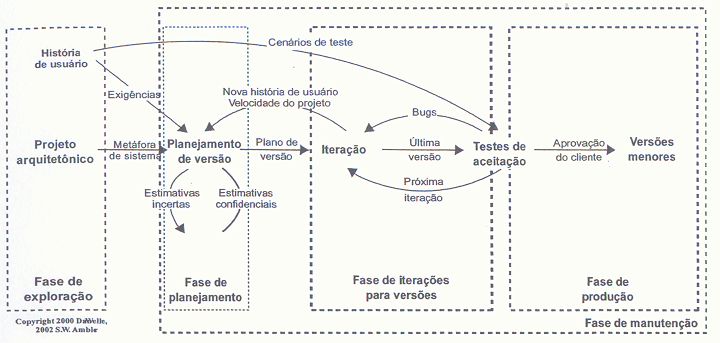
\includegraphics[scale=0.85]{cicloXp.png}
	\caption{Processo	de	desenvolvimento	eXtreme Programming (XP)}
	\label{img1}
\end{figure}

\subsection{Iterações e Artefatos definidos}

A partir dos conceitos descritos e das práticas propostas foi elaborado um plano de desenvolvimento para o projeto onde será destacado os artefato que a metodologia irá gerar juntamente com as atividades adotadas ao longo do desenvolvimento.

Um processo ágil deve ser capaz de administrar a imprevisibilidade, sendo capaz de se adaptar às diversas mudanças que podem ocorrer durante o desenvolvimento do projeto, e essa adaptação deve ser feita de forma incremental, ou seja, o desenvolvedor necessita do feedback.

Os feedbacks podem ser dados através de partes funcionais do sistema (incrementos), as quais são entregues em datas pré estipuladas, possibilitando que as adaptações sejam feitas seguindo o mesmo ritmo das mudanças que podem surgir no decorrer do desenvolvimento.

 Nesse projeto em questão o cliente é a banca avaliadora, este avaliará os limites do software e se estava dentro do nível de aceitação e dará o feedback. Como a metodologia escolhida acaba gerando poucos artefatos e pouca documentação, e interações mais curtas iriam geram problemas no desenvolvimento devido a pouca experiência na aplicação do processo, a solução encontrada foi dividir o projeto em três etapas de desenvolvimento onde as interações propostas foram relatadas no cronograma.
 
A primeira etapa do projeto se inicia com a atividade de “ouvir” e conhecer o modelo de negócio, possibilitando  levantamento de requisitos e levando ao desenvolvedor o entendimento sobre qual o ambiente o software que será desenvolvido vai atuar. Após o levantamento de requisitos, a equipe deu início à criação das histórias de usuário, onde são descritos os resultados, as características e as funcionalidades requisitadas para o software a ser construído, artefatos como casos de uso, diagrama de atividades e diagramas de classes  surgem dessas discussões. Os requisitos que serão responsáveis por criar as história, as quais será atribuído um grau de prioridade, ou seja, a história que receber o grau de prioridade maior é a que deve ser elaborada primeiro. 

O desenvolvedor deve ordenar as histórias de forma que as histórias de maior valor serão deslocadas para cima no cronograma e implementadas primeiro. A metodologia XP permite que novas histórias sejam escritas a qualquer momento e conforme o projeto prossegue, pode-se acrescentar novas histórias, mudar o grau de prioridade, dividi-las ou eliminá-las. 

A segunda etapa trata de um releases do sistema onde será implementado o banco de dados juntamente com o código fonte,  abordando os requisitos baseados nas histórias do consumidor a segunda etapa está amplamente ligada a terceira etapa de desenvolvimento.  Será utilizou como mecanismo para entender o software em uma perspectiva orientada a objetos um artefato proposto pela metodologia, os cartões CRC (classe-responsabilidade-colaborador), juntamente ao diagrama de classes. São apresentadas no cartão CRC o nome da classe, os atributos e métodos (responsabilidades), e as associações (colaboradores).  

Cartão CRC(classe-responsabilidade-colaborador) imagem \ref{img2}: 
 \begin{figure}[h!]
    \centering
	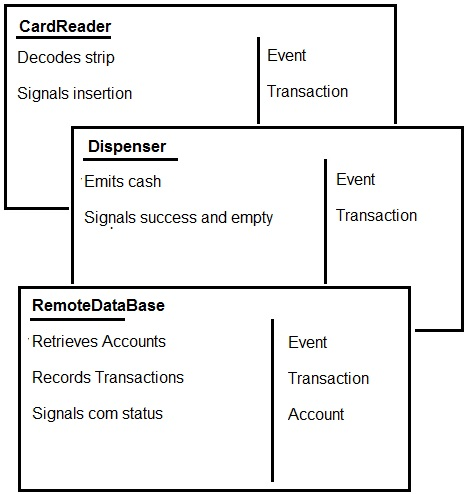
\includegraphics[scale=0.7]{CRC}
	\caption{Cartão CRC(classe-responsabilidade-colaborador)}
	\label{img2}
\end{figure}

Para a atividade de codificação foi utilizado a ferramenta Visual Studio Code, ferramenta de edição de texto livre configurada para as linguagens Node, HTML, JS e Mongo, utilizada para a confecção e manutenção dos arquivos JS e HTML do sistema web, e Google Chrome, ferramenta de interface visual de desenvolvimento disponível.

A terceira etapa se fará presente durante a segunda etapa, se consiste na fase de testes e o desenvolvimento das interfaces, segundo Sommerville (2007) uma das principais características dos testes dentro do XP e o  test-first,  que trata das funcionalidades que serão desenvolvidas assim como trata a interface. Segundo o desenvolvimento test-first a equipe já tem os testes escritos antes mesmo da implementação, sendo um componente executável possibilitando o teste logo após a história ser implementada.


Para a fase de teste tanto das interfaces como o código será utilizado a técnica de Desenvolvimento Orientado a Testes (TDD, em inglês Test Driven Development)	se baseia em pequenos ciclos de repetições, onde para cada funcionalidade do sistema um teste é criado antes. Este novo teste criado inicialmente falha, já que ainda não foi implementada da funcionalidade em questão e, em seguida, é implementada a funcionalidade para fazer o teste passar. Mais antes de aprovar o teste é necessário que a funcionalidade criada seja refatorada, isto é deve se aplicar as práticas do XP ao código, como limpar partes desnecessárias e dar coesão ao código.  

Ciclo do TDD imagem \ref{img2}: 
 \begin{figure}[h!]
    \centering
	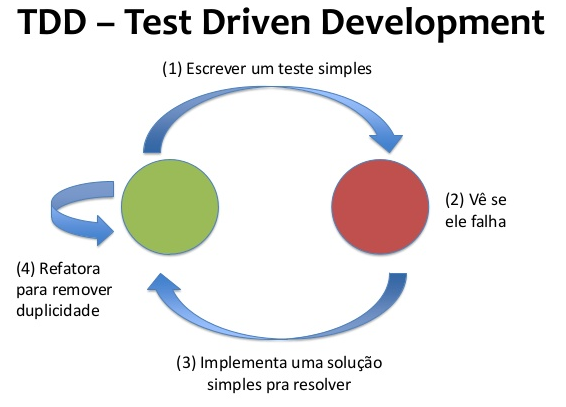
\includegraphics[scale=0.7]{tdd}
	\caption{Ciclo do TDD}
	\label{img2}
\end{figure}

Assim com testes de unidade a metodologia prevê testes de aceitação também denominadas testes de clientes que serão feitas a partir das entregas feitas ao professor. Os testes são a garantia que o sistema está sendo desenvolvido de acordo com os requisitos propostos.


Para o registro de atividades e controle de interações será utilizado uma ferramenta de gestão a Trello, que ajuda a organização do grupo quanto ao andamento do desenvolvimento assim como mantém o andamento do projeto dentro do cronograma proposto.


\chapter{Proximas Atividades}
\section{Cronograma}
Cronograma Previsto para o desenvolvimento, tabela \ref{tab1}:
\begin{table}[h!]
\caption{Tabela cronogram previsto}
\label{tab1}
\begin{tabular}{|l|l|}
\hline
\textbf{Interações}                                                                                                                                                  & \textbf{Data inicio / Data da Entrega} \\ \hline
\begin{tabular}[c]{@{}l@{}}Analise de requisitos - Levantamento das \\ Histórias dos Usuário \\ ( Requisitos funcionais e não funcionais dos Usuários )\end{tabular} & 20/11/2018 à 10/01/2019                \\ \hline
Elaboração dos diagramas de Caso de Uso                                                                                                                              & 10/01/2019 à 10/03/2019                \\ \hline
Elaboração dos diagramas de atividade                                                                                                                                & 10/01/2019 à 10/03/2019                \\ \hline
\begin{tabular}[c]{@{}l@{}}Elaboração do modelo conceitual e \\ logico do banco de dados\end{tabular}                                                                & 10/01/2019 à 10/03/2019                \\ \hline
Elaboração dos diagrama de Classe                                                                                                                                    & 10/01/2019 à 10/03/2019                \\ \hline
Elaboração do dicionário de dados                                                                                                                                    & 10/01/2019 à 10/03/2019                \\ \hline
Revisão de acordo com o feedback                                                                                                                                     & 11/03/2019 à 11/04/2019                \\ \hline
Elaboração dos cartões CRC                                                                                                                                           & 11/04/2019 à 11/05/2019                \\ \hline
Implementação das Classes e fase de Testes                                                                                                                           & 11/04/2019 à 11/05/2019                \\ \hline
Revisão e ajustes                                                                                                                                                    & 12/05/2019 à 01/06/2018                \\ \hline
Reservado para ajustar de acordo com o  feedback                                                                                                                     & 02/06/2019 à 30/06/2019                \\ \hline
\end{tabular}
\end{table}

%bibliografia usando o bibtex
%Para se editar a bibliografia deve-se editar o arquivo biblio.bib, que pode ser feito através de um editor padão do latex ou até do bloco de notas(não recomendo).
\bibliographystyle{abnt}
\bibliography{biblio}
\end{document}